\documentclass[12pt,a4paper]{article}

% =========================
% PAQUETES
% =========================
\usepackage[utf8]{inputenc}
\usepackage[T1]{fontenc}
\usepackage[spanish, es-nodecimaldot]{babel}
\usepackage{lmodern}
\usepackage{geometry}
\geometry{margin=2.5cm}
\usepackage{setspace}
\usepackage{amsmath, amssymb, amsfonts}
\usepackage{graphicx}
\usepackage{float}
\usepackage{booktabs}
\usepackage{array}
\usepackage{longtable}
\usepackage{enumitem}
\usepackage{xcolor}
\usepackage{hyperref}
\usepackage{listings}
\usepackage{caption}
\usepackage{subcaption}
\usepackage{fancyhdr}
\usepackage{multirow}
\usepackage{forest}

\hypersetup{
    colorlinks=true,
    linkcolor=blue,
    urlcolor=blue,
    citecolor=blue
}

\pagestyle{fancy}
\fancyhf{}
\fancyhead[L]{TE3002B - Machine Learning}
\fancyhead[R]{Reto Ridge Regression}
\fancyfoot[C]{\thepage}

\setstretch{1.15}

% =========================
% CONFIGURACIÓN DE CÓDIGO
% =========================
\lstset{
    language=Python,
    basicstyle=\ttfamily\small,
    keywordstyle=\color{blue},
    commentstyle=\color{green!50!black},
    stringstyle=\color{red!70!black},
    breaklines=true,
    frame=single,
    showstringspaces=false,
    tabsize=4
}

% =========================
% DATOS
% =========================
\title{\textbf{Reto: Ridge Regression (L2) --- Reconocimiento Facial con Imágenes Reales}\\
\vspace{0.3cm}
\large Reporte técnico}
\author{
Equipo 4 \\
Integrantes: \\
Oscar Carranza Hernández \hspace{0.5cm} | A00838649\\
Valentina Gonzalez Benedossi \hspace{0.5cm} | A00839507\\
Ricardo Gaspar Ochoa \hspace{0.5cm} | A00838841\\
Rhett Nieto Ramírez \hspace{0.5cm} | A01286100
}
\date{\today}

% =========================
% DOCUMENTO
% =========================
\begin{document}

\maketitle
\thispagestyle{empty}

\vspace{0.5cm}

\begin{abstract}
En este trabajo se implementó un clasificador de reconocimiento facial basado en Ridge Regression multivariado. El pipeline desarrollado incluye carga del dataset, preprocesamiento de imágenes, partición estratificada en conjuntos de entrenamiento, validación y prueba, normalización, reducción de dimensionalidad mediante PCA, codificación de clases con un símplex regular y clasificación por distancia mínima al vértice más cercano. Adicionalmente, se realizó una etapa de limpieza de imágenes reales mediante detección y recorte de rostro. Se presentan las partes completadas, los resultados obtenidos y una reflexión sobre los criterios aún pendientes con base en la rúbrica de evaluación.
\end{abstract}

\newpage
\tableofcontents
\newpage

% =========================
\section{Introducción}
% =========================
El objetivo del reto es implementar un clasificador de reconocimiento facial usando Ridge Regression multivariado, siguiendo la lógica del pipeline descrito en la actividad. El problema consiste en representar cada identidad facial dentro de un espacio de salida continuo y regularizado, de forma que la predicción final se obtenga como el vértice más cercano de un símplex regular.

En nuestro caso, el desarrollo realizado se enfocó en:
\begin{itemize}
    \item cargar y preprocesar imágenes en escala de grises,
    \item dividir el conjunto de datos en entrenamiento, validación y prueba de manera estratificada,
    \item normalizar usando únicamente estadísticas del conjunto de entrenamiento,
    \item aplicar PCA para reducir dimensionalidad,
    \item implementar Ridge Regression manualmente,
    \item buscar el mejor hiperparámetro $\alpha$,
    \item clasificar por distancia mínima en el espacio del símplex,
    \item analizar resultados mediante MSE, ridge path, matriz de confusión y ejemplos visuales,
    \item y limpiar imágenes reales mediante recorte automático de rostro.
\end{itemize}

También se identifican explícitamente las partes que todavía no cumplen completamente con la rúbrica, con el fin de presentar una entrega honesta, ejecutable y bien justificada.

% =========================
\section{Eje 1 --- Diseño y teoría}
% =========================

\subsection{Motivación: multicolinealidad en imágenes}
En problemas de clasificación con imágenes, es común que exista alta correlación entre variables de entrada, especialmente entre píxeles vecinos. Esto provoca multicolinealidad, ya que varias características contienen información redundante o muy similar. Como consecuencia, la matriz $X^\top X$ puede volverse mal condicionada o cercana a singular.

En este contexto, usar mínimos cuadrados ordinarios (OLS) puede ser problemático porque pequeñas perturbaciones en los datos pueden producir cambios muy grandes en los coeficientes estimados. Esto genera alta varianza en el modelo, inestabilidad numérica y menor capacidad de generalización.

\subsection{Por qué OLS falla cuando $X^\top X$ es casi singular}
El estimador de OLS se expresa como:
\[
\hat{\beta}_{OLS} = (X^\top X)^{-1}X^\top y
\]
Si $X^\top X$ es singular o casi singular, su inversa no existe o es numéricamente inestable. Esto provoca:
\begin{itemize}
    \item coeficientes muy grandes,
    \item sensibilidad extrema al ruido,
    \item predicciones erráticas,
    \item sobreajuste.
\end{itemize}

Ridge Regression corrige este problema añadiendo un término de regularización:
\[
\hat{\beta}_{Ridge} = (X^\top X + \alpha I)^{-1}X^\top y
\]
donde $\alpha > 0$ desplaza los autovalores de $X^\top X$ y mejora la estabilidad de la inversión.

\subsection{Derivación de Ridge Regression}
La función objetivo de Ridge es:
\[
J(\beta) = \|y - X\beta\|_2^2 + \alpha \|\beta\|_2^2
\]

Expandiendo:
\[
J(\beta) = (y - X\beta)^\top (y - X\beta) + \alpha \beta^\top \beta
\]

\[
J(\beta) = y^\top y - 2\beta^\top X^\top y + \beta^\top X^\top X \beta + \alpha \beta^\top \beta
\]

Derivando respecto a $\beta$:
\[
\frac{\partial J}{\partial \beta} = -2X^\top y + 2X^\top X \beta + 2\alpha \beta
\]

Igualando a cero:
\[
-2X^\top y + 2X^\top X \beta + 2\alpha \beta = 0
\]

\[
X^\top X \beta + \alpha \beta = X^\top y
\]

\[
(X^\top X + \alpha I)\beta = X^\top y
\]

Por lo tanto:
\[
\hat{\beta}_{Ridge} = (X^\top X + \alpha I)^{-1}X^\top y
\]

\subsection{Interpretación geométrica}
Geométricamente, Ridge Regression puede interpretarse como minimizar el error cuadrático sujeto a una restricción sobre la norma de $\beta$:
\[
\|\beta\|_2^2 \leq c
\]
Esto significa que la solución está restringida a una región esférica. La regularización hace que la solución tienda a valores de menor magnitud, reduciendo la varianza del modelo y favoreciendo soluciones más estables.

\subsection{Símplex regular y clasificación}
En lugar de codificar las clases con vectores one-hot, se usa un símplex regular, donde cada identidad se representa como un vértice equidistante de los demás. Esto permite una representación más geométrica y simétrica del problema de clasificación multiclase.

Si hay $m$ clases, se construyen $m$ vértices en $\mathbb{R}^{m-1}$. Cada clase se asocia a uno de esos vértices y la predicción final se realiza encontrando el vértice más cercano a la salida continua del modelo.

La regla de decisión es:
\[
\hat{y} = \arg\min_j \| \hat{Y} - T_j \|_2
\]
donde $T_j$ es el vértice del símplex asociado a la clase $j$.

\subsection{Pipeline implementado}
El pipeline realizado en este trabajo fue:
\[
\text{Imagen} \rightarrow \text{Resize/Blur/EqualizeHist} \rightarrow \text{Vector} \rightarrow \text{Normalización} \rightarrow \text{PCA} \rightarrow \text{Ridge} \rightarrow \text{Símplex} \rightarrow \text{Clase predicha}
\]

\subsection{Bias-variance tradeoff}
El parámetro $\alpha$ controla el compromiso entre sesgo y varianza:
\begin{itemize}
    \item Si $\alpha \to 0$, el modelo se parece a OLS: bajo sesgo pero alta varianza.
    \item Si $\alpha$ crece demasiado, los coeficientes se encogen excesivamente: baja varianza pero alto sesgo.
\end{itemize}

Por ello, se realizó una búsqueda sobre distintos valores de $\alpha$ en escala logarítmica y se seleccionó el que minimizó el error cuadrático medio.

% =========================
\section{Eje 2 --- Programación}
% =========================

\subsection{Descripción general del código}
Se desarrollaron dos scripts principales:
\begin{enumerate}
    \item Un script para clasificación facial con Ridge Regression.
    \item Un script para limpieza de imágenes reales mediante detección y recorte de rostro.
\end{enumerate}

\subsection{Preprocesamiento de imágenes}
Cada imagen se procesa de la siguiente forma:
\begin{enumerate}
    \item redimensionado a $32\times32$,
    \item filtro Gaussiano,
    \item ecualización de histograma.
\end{enumerate}

La función usada fue:

\begin{lstlisting}
def preprocess(img):
    img = cv2.resize(img, (IMG_SIZE, IMG_SIZE))
    img = cv2.GaussianBlur(img, (3,3), 0)
    img = cv2.equalizeHist(img)
    return img
\end{lstlisting}

\subsection{Descripción del dataset real}
En lugar de utilizar el generador sintético incluido en el código de referencia, en este trabajo se utilizó un dataset de imágenes faciales reales organizado por identidad. Cada carpeta del dataset corresponde a una clase distinta, y contiene múltiples imágenes del mismo sujeto bajo condiciones similares de captura.

La estructura general del dataset fue la siguiente:

\begin{forest}
for tree={font=\ttfamily, grow'=0}
[dataset
  [identidad\_0]
  [identidad\_1]
  [identidad\_2]
  [...]
  [identidad\_n]
]
\end{forest}

La Tabla~\ref{tab:dataset_resumen} resume la cantidad de imágenes disponibles por identidad.

\begin{table}[H]
\centering
\caption{Resumen del dataset utilizado.}
\label{tab:dataset_resumen}
\begin{tabular}{lc}
\toprule
\textbf{Identidad} & \textbf{Número de imágenes} \\
\midrule
Identidad 0 & 63 \\
Identidad 1 & 65 \\
Identidad 2 & 62 \\
Identidad 3 & 65 \\
Identidad 4 & 60 \\
Identidad 5 & 61 \\
Identidad 6 & 62 \\
Identidad 7 & 62 \\
Identidad 8 & 62 \\
\bottomrule
\end{tabular}
\end{table}

Si bien el código de referencia del profesor incluía una etapa de generación de dataset sintético a partir de prototipos paramétricos y rasterización de rostros, en esta implementación se decidió trabajar con imágenes faciales reales. Por esta razón, no se integró la generación sintética dentro del pipeline final de entrenamiento. No obstante, se conservó la lógica central del método de clasificación mediante Ridge Regression multivariado y codificación de clases con símplex regular.

\subsection{Partición train/validation/test}
El conjunto de datos se dividió en tres subconjuntos estratificados con semilla reproducible:
\begin{itemize}
    \item entrenamiento,
    \item validación,
    \item prueba.
\end{itemize}

Primero se separó el 20\% de las imágenes para prueba. Posteriormente, el 80\% restante se dividió en entrenamiento y validación. De esta forma, el conjunto de validación se utilizó para seleccionar el hiperparámetro $\alpha$, mientras que el conjunto de prueba se reservó exclusivamente para la evaluación final del modelo.

\begin{lstlisting}
X_trainval, X_test, y_trainval, y_test = train_test_split(
    X, y,
    test_size=0.2,
    stratify=y,
    random_state=42
)

X_train, X_val, y_train, y_val = train_test_split(
    X_trainval, y_trainval,
    test_size=0.2,
    stratify=y_trainval,
    random_state=42
)
\end{lstlisting}

Este esquema garantiza que el conjunto de prueba permanezca completamente separado durante la selección de hiperparámetros, evitando fuga de información y cumpliendo con la recomendación metodológica de la rúbrica.

\subsection{Normalización}
La media y desviación estándar se calcularon únicamente con el conjunto de entrenamiento:

\begin{lstlisting}
mu = X_train.mean(axis=0)
sigma = X_train.std(axis=0) + 1e-8

X_train = (X_train - mu) / sigma
X_val   = (X_val   - mu) / sigma
X_test  = (X_test  - mu) / sigma
\end{lstlisting}

Esto evita fuga de información del conjunto de validación y del conjunto de prueba.

\subsection{Reducción de dimensionalidad con PCA}
Para disminuir el número de variables, se aplicó PCA usando SVD:

\begin{lstlisting}
k = min(120, X_train.shape[0] - 1)

U, S, Vt = np.linalg.svd(X_train, full_matrices=False)
W = Vt[:k]

X_train = X_train @ W.T
X_val   = X_val @ W.T
X_test  = X_test @ W.T
\end{lstlisting}

\subsection{Construcción del símplex regular}
Cada clase se codificó como un vértice de un símplex regular:

\begin{lstlisting}
def simplex_regular(m):
    T = np.zeros((m, m - 1))
    T[0, 0] = 1.0
    for i in range(1, m):
        T[i, 0] = -1.0 / (m - 1)
    for k in range(1, m - 1):
        T[k, k] = np.sqrt(1 - np.sum(T[k, :k]**2))
        for i in range(k + 1, m):
            T[i, k] = -T[k, k] / (m - k - 1)
    return T
\end{lstlisting}

\subsection{Implementación manual de Ridge}
La implementación se hizo manualmente usando la ecuación cerrada y \texttt{np.linalg.solve}, sin utilizar \texttt{sklearn.Ridge}:

\begin{lstlisting}
def ridge_regression(X, Y, alpha):
    I = np.eye(X.shape[1])
    return np.linalg.solve(X.T @ X + alpha * I, X.T @ Y)
\end{lstlisting}

\subsection{Búsqueda del mejor $\alpha$}
Se probaron 50 valores de $\alpha$ en escala logarítmica. A diferencia de la versión inicial, la selección del hiperparámetro ya no se realizó sobre el conjunto de prueba, sino sobre el conjunto de validación.

\begin{lstlisting}
for a in alphas:
    beta = ridge_regression(X_train, Y_train, a)
    Y_val_pred = X_val @ beta
    mse = np.mean((Y_val_pred - T[y_val])**2)
    mse_list.append(mse)
\end{lstlisting}

Una vez seleccionado el valor óptimo de $\alpha$, el desempeño final del clasificador se reportó únicamente sobre el conjunto de prueba.

\subsection{Clasificación}
La clase final se determina por la menor distancia euclidiana al vértice del símplex:

\begin{lstlisting}
def predict_class(Y_pred, T):
    dists = np.linalg.norm(Y_pred[:, None] - T[None, :], axis=2)
    return np.argmin(dists, axis=1)
\end{lstlisting}

\subsection{Métricas y visualizaciones}
Se obtuvieron:
\begin{itemize}
    \item accuracy,
    \item curva MSE vs $\alpha$,
    \item ridge path,
    \item matriz de confusión normalizada,
    \item visualización de predicciones correctas e incorrectas.
\end{itemize}

\subsection{Resultados}
En esta sección deben insertarse las figuras obtenidas por el código.

\begin{figure}[H]
    \centering
    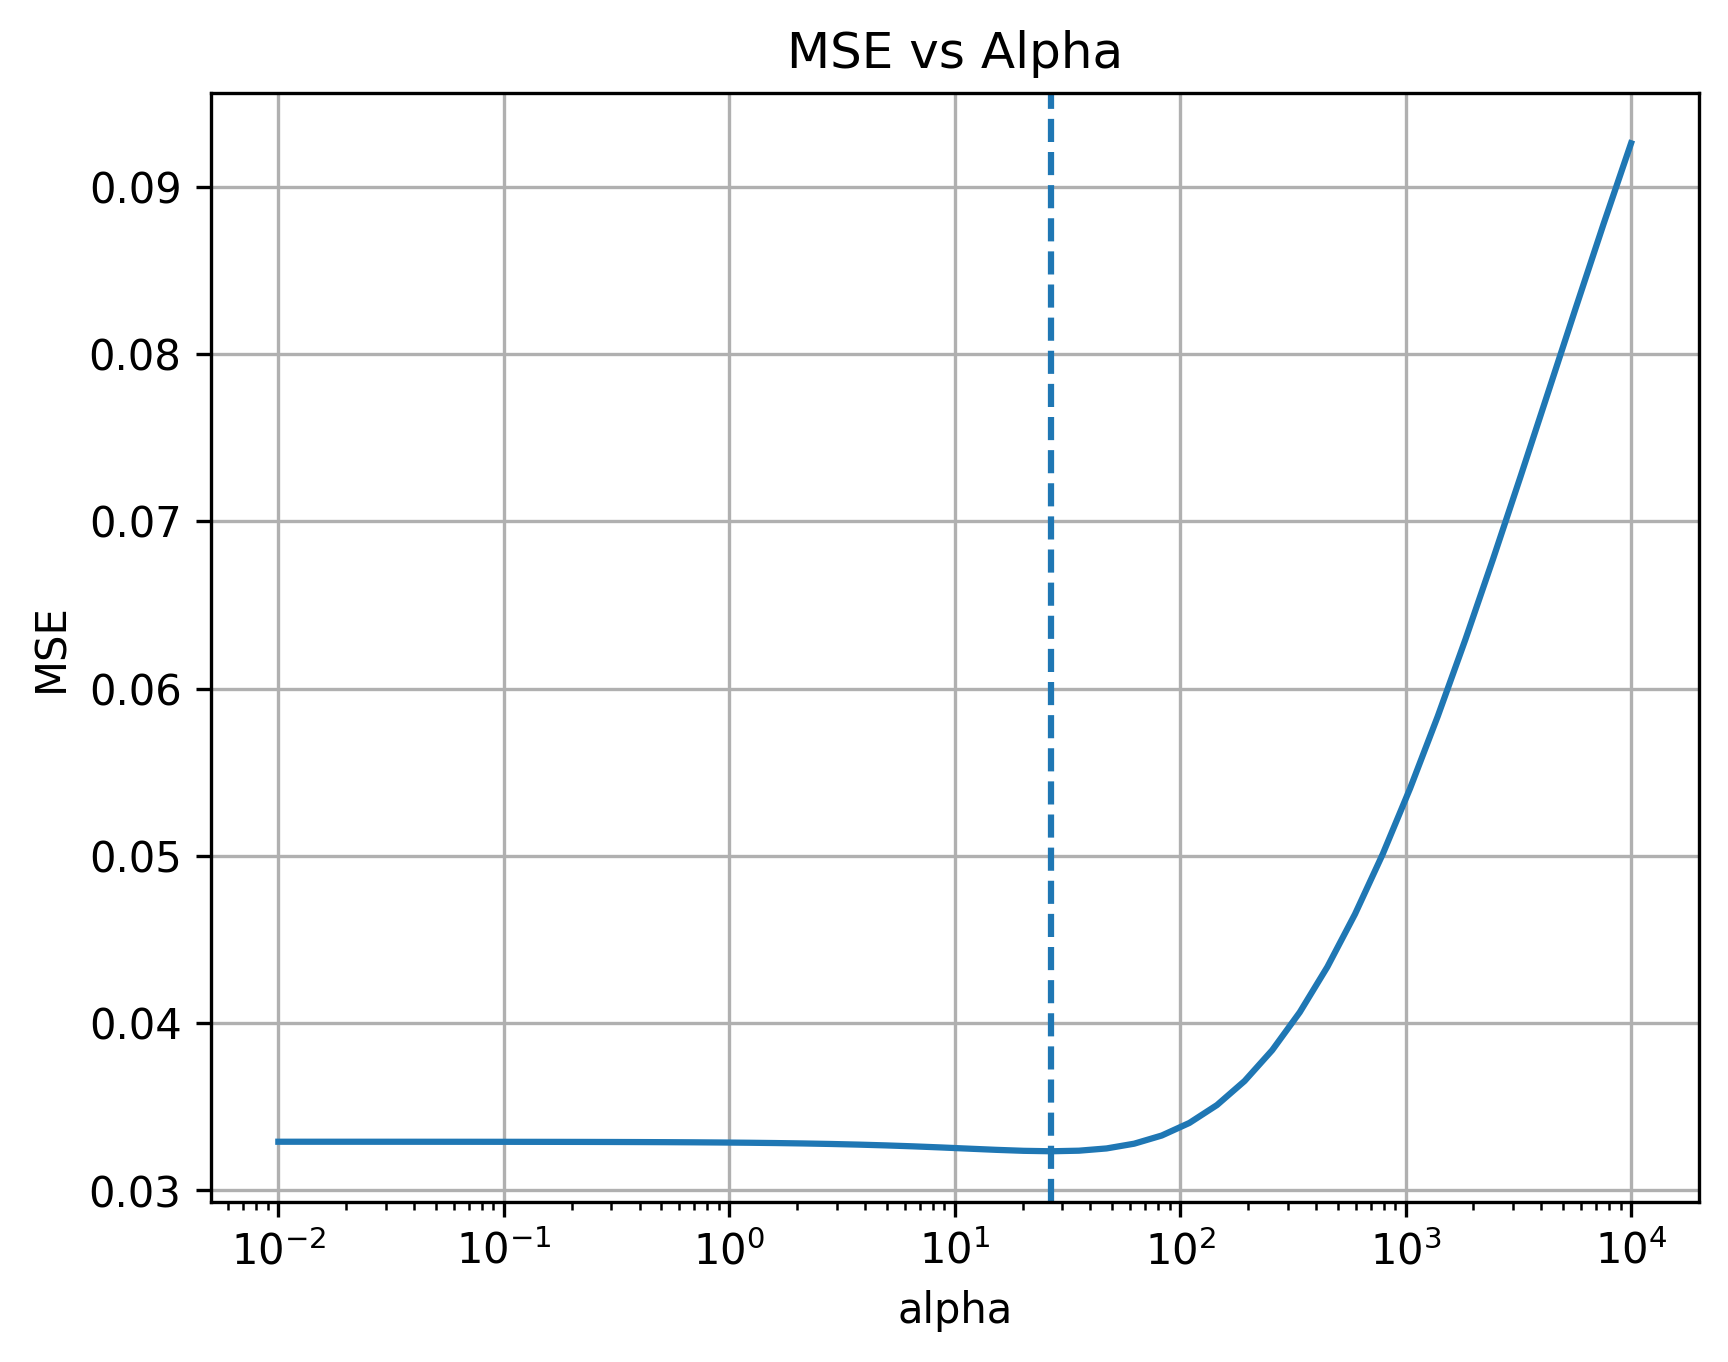
\includegraphics[width=0.7\textwidth]{mse_vs_alpha.png}
    \caption{Curva MSE vs $\alpha$ sobre validación.}
    \label{fig:mse_alpha}
\end{figure}

\begin{figure}[H]
    \centering
    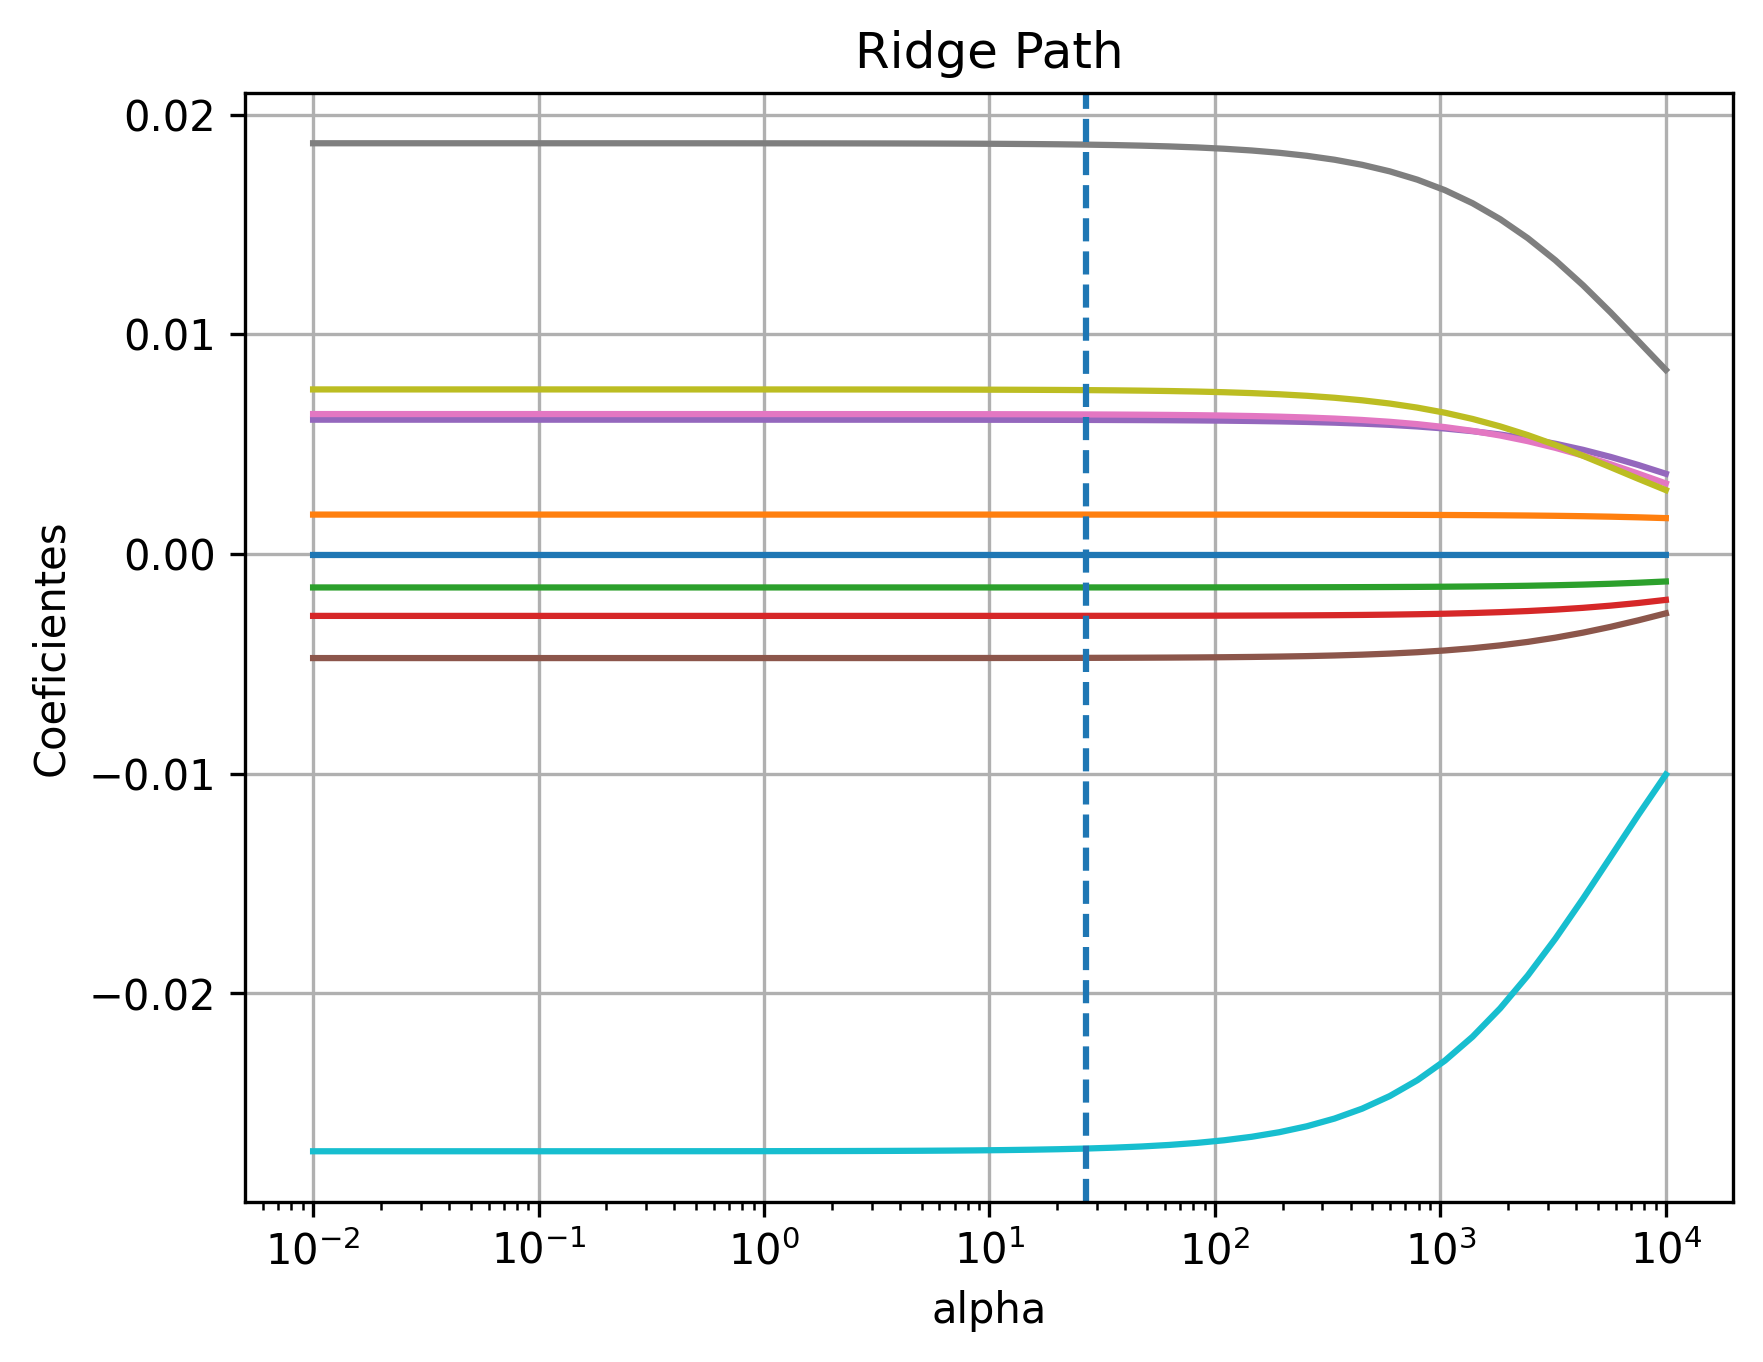
\includegraphics[width=0.7\textwidth]{ridge_path.png}
    \caption{Ridge path para distintos valores de $\alpha$.}
    \label{fig:ridge_path}
\end{figure}

\begin{figure}[H]
    \centering
    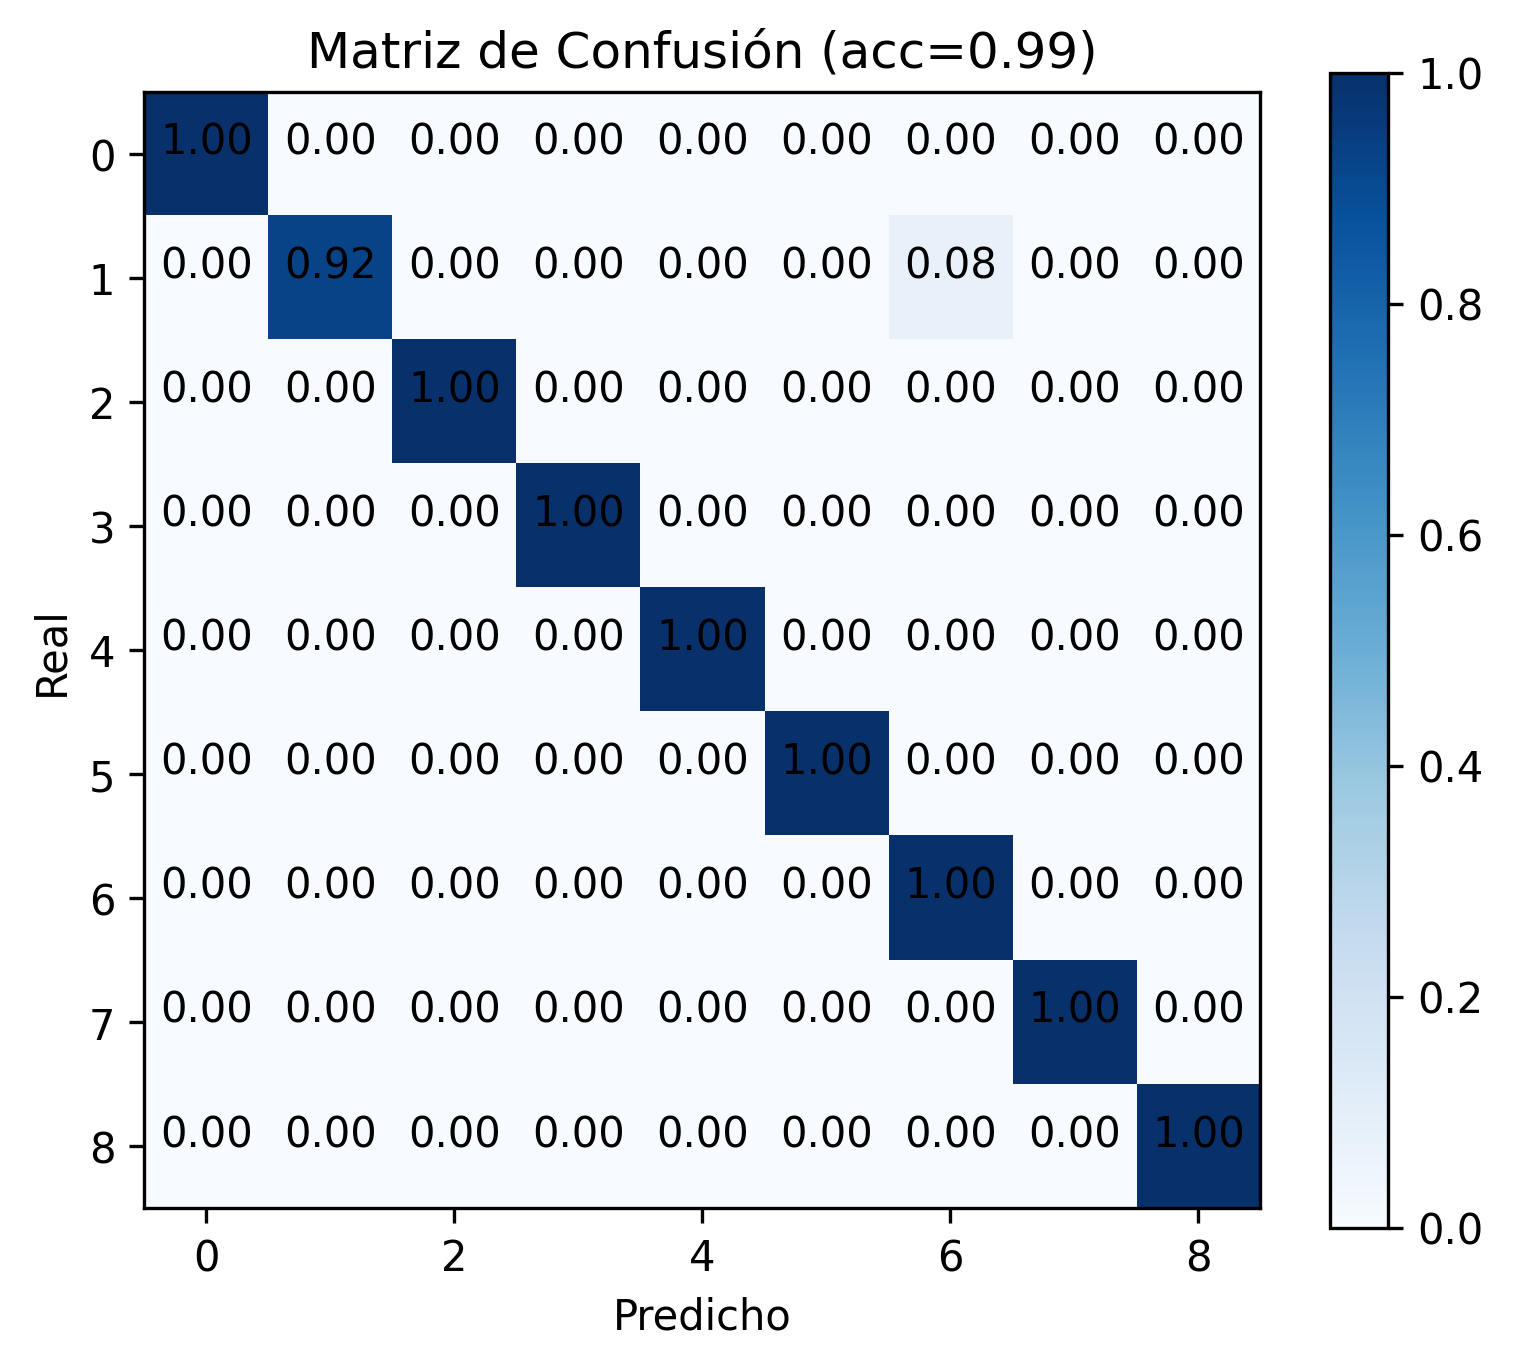
\includegraphics[width=0.6\textwidth]{confusion_matrix.png}
    \caption{Matriz de confusión normalizada del conjunto de prueba.}
    \label{fig:conf_matrix}
\end{figure}

\begin{figure}[H]
    \centering
    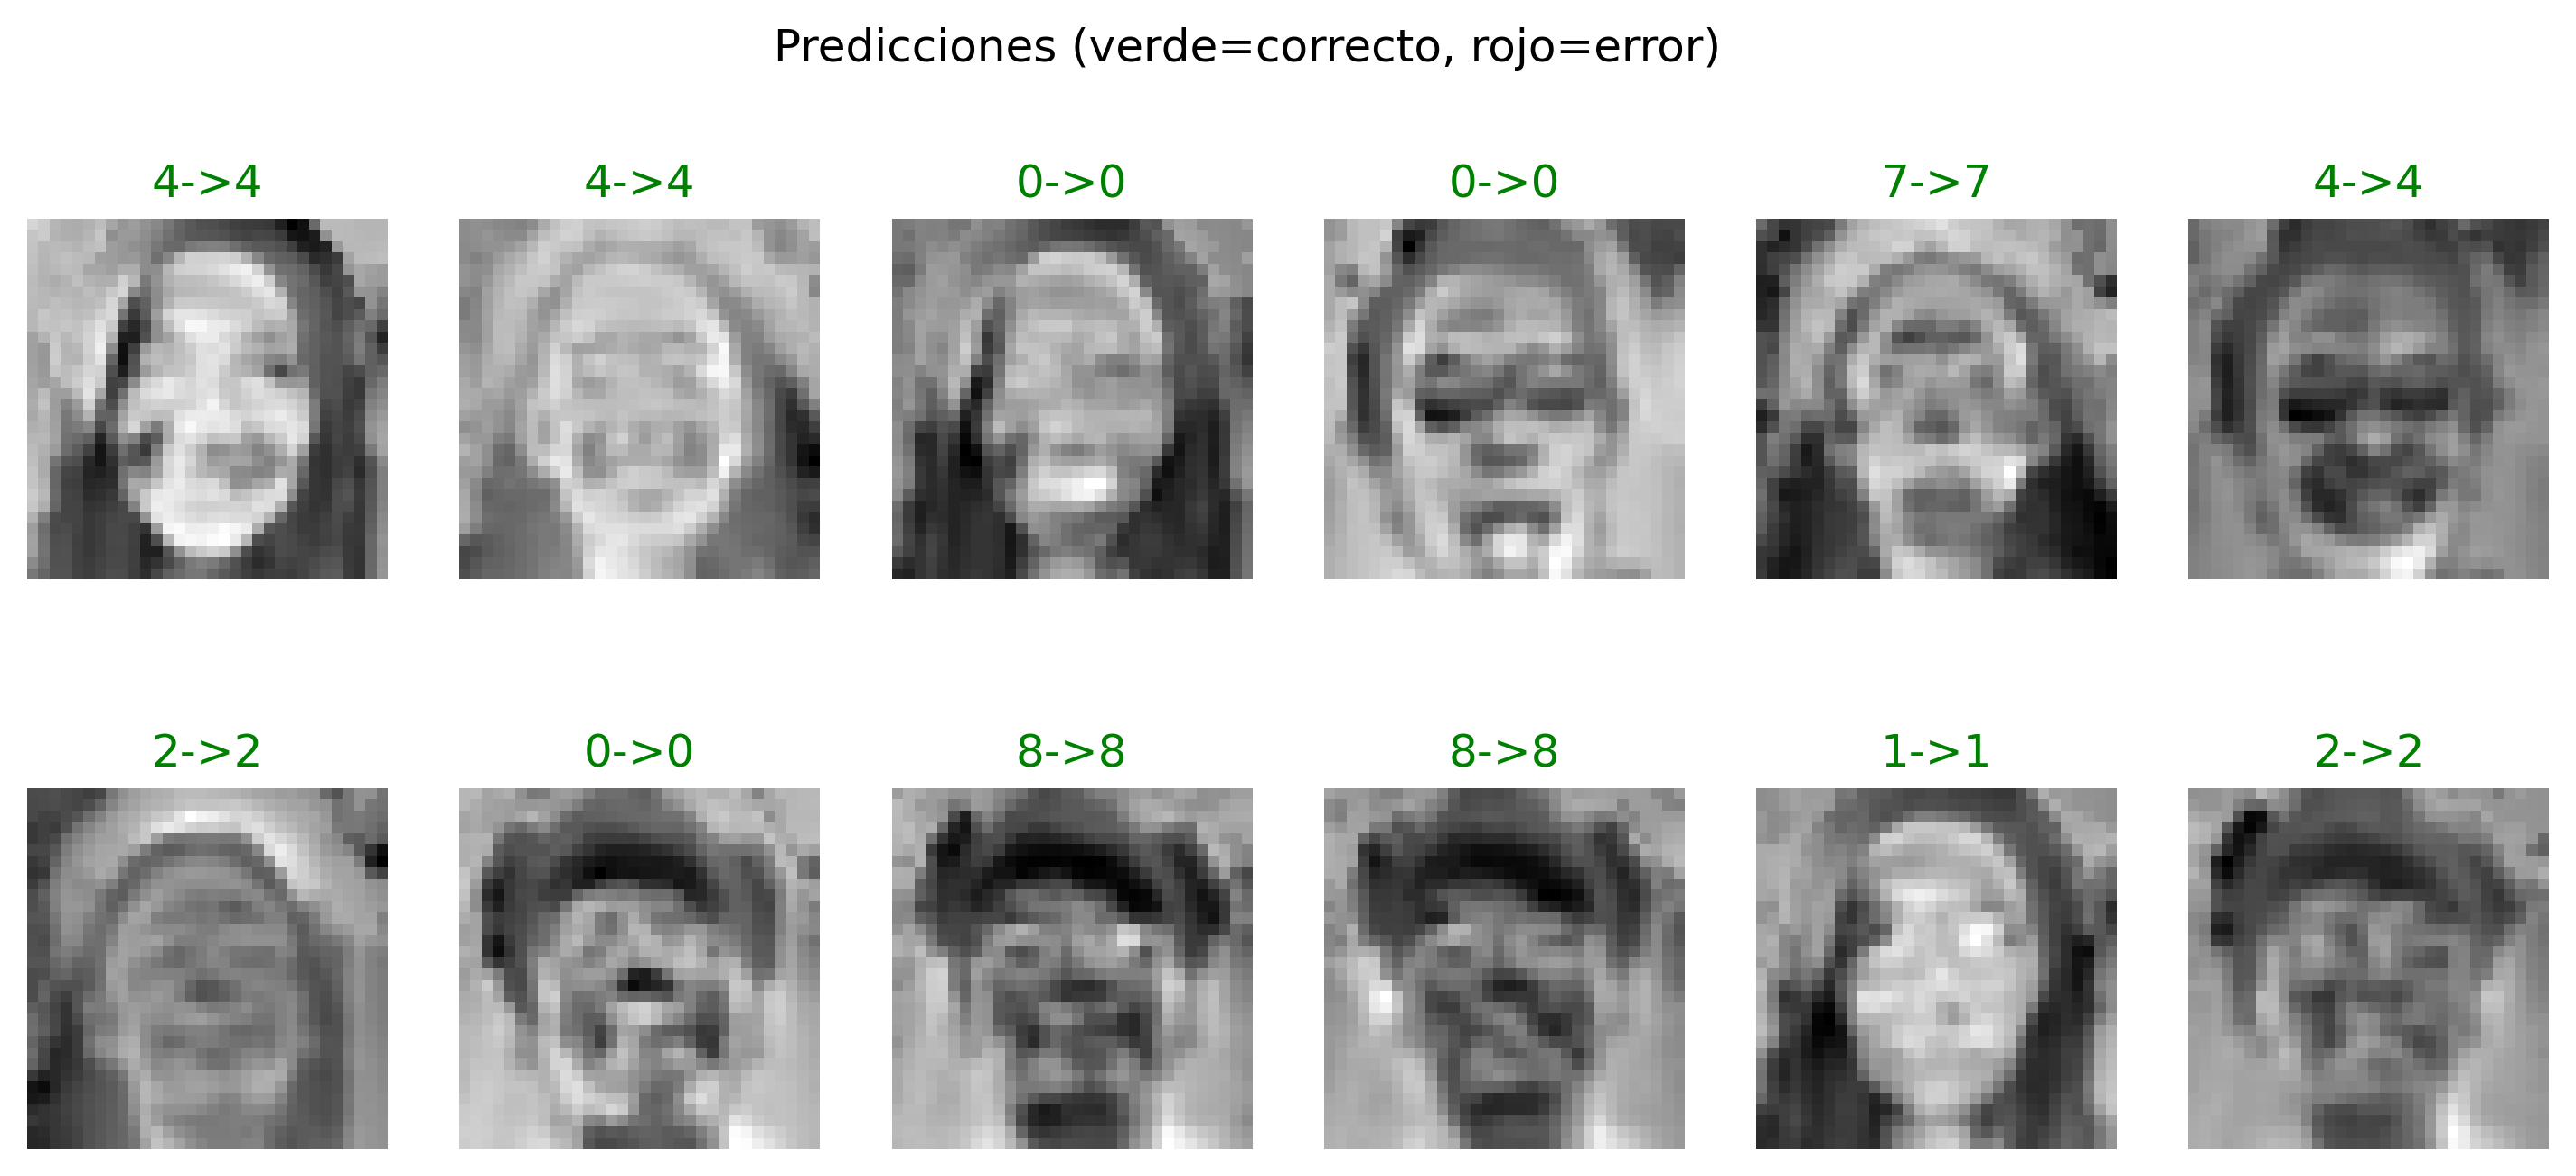
\includegraphics[width=\textwidth]{predicciones.png}
    \caption{Ejemplos de predicciones en el conjunto de prueba. Verde: correcto. Rojo: error.}
    \label{fig:predicciones}
\end{figure}

\subsection{Análisis de resultados}
La matriz de confusión permite identificar qué identidades tienden a confundirse más. En general, las confusiones pueden deberse a similitud en rasgos faciales, baja resolución de las imágenes o pérdida de información tras la reducción con PCA.

Aquí conviene agregar un análisis puntual con base en la matriz de confusión obtenida. Por ejemplo, si dos identidades presentan mayor número de errores cruzados, una posible hipótesis es que comparten patrones de iluminación, pose o estructura facial similares, lo que produce representaciones cercanas en el espacio reducido.

\subsection{Calidad del código}
El código se estructuró en funciones separadas para:
\begin{itemize}
    \item preprocesamiento,
    \item carga del dataset,
    \item construcción del símplex,
    \item Ridge Regression,
    \item predicción de clase,
    \item recorte de rostro.
\end{itemize}

Sin embargo, como mejora pendiente:
\begin{itemize}
    \item faltan docstrings formales en varias funciones,
    \item faltan algunos experimentos adicionales requeridos por la rúbrica,
    \item conviene eliminar dependencias no esenciales si se busca una implementación todavía más minimalista.
\end{itemize}

% =========================
\section{Eje 3 --- Captura fotográfica y limpieza de datos}
% =========================

\subsection{Objetivo}
Además del clasificador, se desarrolló un script para procesar imágenes reales y recortar automáticamente la región facial antes de usarlas en el pipeline.

\subsection{Protocolo de captura}
Para la adquisición de imágenes reales se definió un protocolo de captura con el objetivo de mantener consistencia entre identidades y reducir variaciones no deseadas. Se procuró utilizar un fondo uniforme, una distancia aproximadamente constante entre cámara y sujeto, y una pose predominantemente frontal. Asimismo, se buscó mantener iluminación lo más homogénea posible y evitar oclusiones importantes del rostro.

La Figura~\ref{fig:setup_captura} muestra ejemplos del setup utilizado durante la adquisición de imágenes.

\begin{figure}[H]
    \centering
    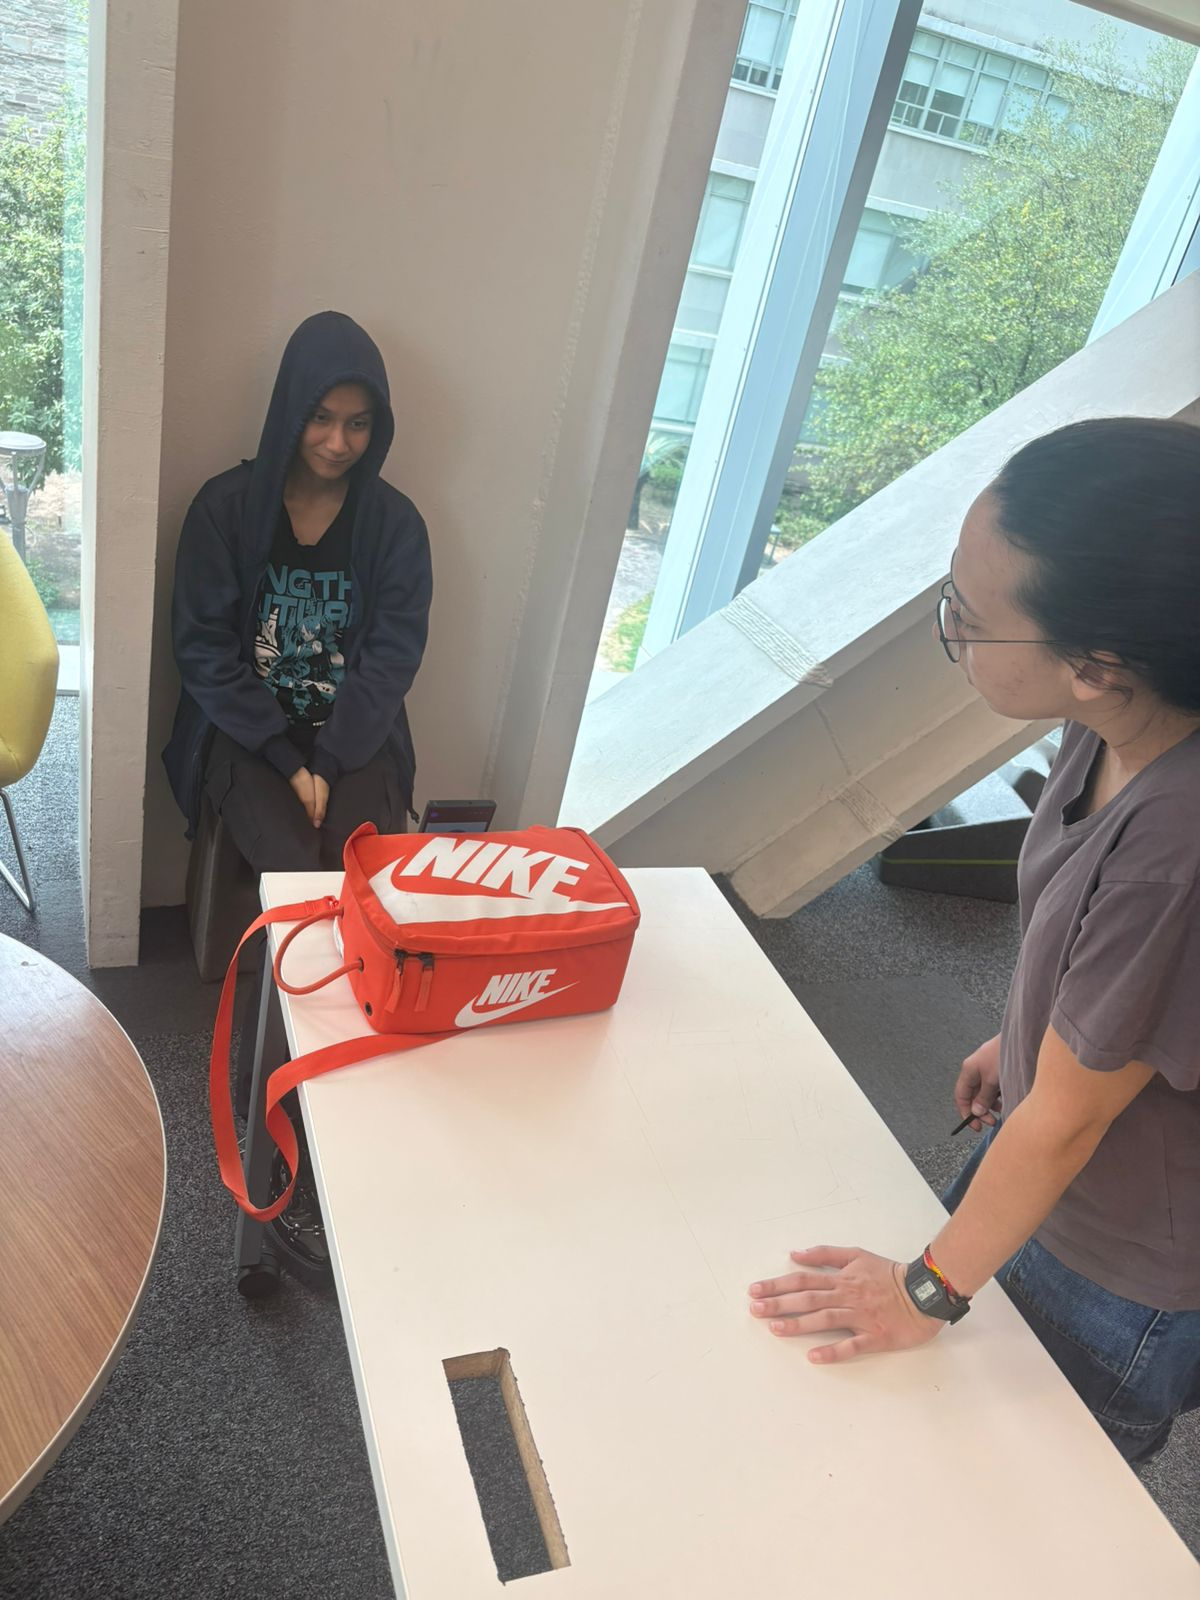
\includegraphics[width=0.65\textwidth]{setup.jpeg}
    \caption{Protocolo de captura utilizado para la adquisición de imágenes reales.}
    \label{fig:setup_captura}
\end{figure}

\subsection{Detección y recorte de rostro}
Se utilizó un clasificador Haar Cascade para detectar caras y recortar la más grande encontrada en la imagen.

\begin{lstlisting}
face_cascade = cv2.CascadeClassifier(
    cv2.data.haarcascades + "haarcascade_frontalface_default.xml"
)
\end{lstlisting}

La función principal fue:

\begin{lstlisting}
def recortar_cara(img):
    gray = cv2.cvtColor(img, cv2.COLOR_BGR2GRAY)

    faces = face_cascade.detectMultiScale(
        gray,
        scaleFactor=1.2,
        minNeighbors=5,
        minSize=(50, 50)
    )

    if len(faces) == 0:
        return None

    x, y, w, h = sorted(faces, key=lambda f: f[2]*f[3], reverse=True)[0]

    pad = int(0.2 * w)
    x1 = max(x - pad, 0)
    y1 = max(y - pad, 0)
    x2 = min(x + w + pad, img.shape[1])
    y2 = min(y + h + pad, img.shape[0])

    face = img[y1:y2, x1:x2]
    return face
\end{lstlisting}

\subsection{Conversión y almacenamiento}
Después del recorte:
\begin{enumerate}
    \item se convierte a escala de grises,
    \item se redimensiona a $32\times32$,
    \item se guarda la imagen resultante.
\end{enumerate}

\begin{lstlisting}
face_gray = cv2.cvtColor(face, cv2.COLOR_BGR2GRAY)
face_resized = cv2.resize(face_gray, (SIZE, SIZE))
cv2.imwrite(out_path, face_resized)
\end{lstlisting}

\subsection{Resultados del filtrado}
El script también contabiliza cuántas imágenes fueron detectadas correctamente y cuántas fallaron.

\begin{lstlisting}
print(f"Caras detectadas: {count_ok}")
print(f"Fallos: {count_fail}")
\end{lstlisting}

\subsection{Registro de imágenes descartadas}
Como parte del control de calidad del dataset, se generó un archivo en formato CSV con el registro de imágenes descartadas durante la limpieza. Para cada archivo eliminado se almacenó el nombre del archivo, la razón principal del descarte y la fecha de registro.

La Tabla~\ref{tab:descartadas} muestra un ejemplo representativo del log generado.

\begin{table}[H]
\centering
\caption{Ejemplo del registro de imágenes descartadas.}
\label{tab:descartadas}
\begin{tabular}{lll}
\toprule
\textbf{Archivo} & \textbf{Razón} & \textbf{Fecha} \\
\midrule
img\_014.jpg & Rostro no detectado & 2026-04-17 \\
img\_027.jpg & Imagen borrosa & 2026-04-17 \\
img\_043.jpg & Encuadre incorrecto & 2026-04-17 \\
\bottomrule
\end{tabular}
\end{table}

Además, el archivo \texttt{imagenes\_descartadas.csv} se incluyó como evidencia del proceso de limpieza y trazabilidad de los datos.

El archivo completo puede consultarse en el repositorio del proyecto:
\url{https://github.com/Cuper245/modulo3-munoz}

\subsection{Limitaciones frente a la rúbrica}
Aunque el pipeline principal del clasificador está completo, aún existen algunas extensiones posibles para mejorar el cumplimiento total de la rúbrica:

\begin{itemize}
    \item el recorte no usa landmarks de ojos, nariz y barbilla,
    \item no se muestran histogramas antes/después de la normalización,
    \item no se implementó aumento de datos controlado,
    \item no se realizó el experimento de sensibilidad al nivel de ruido $\sigma$,
    \item no se integró la generación sintética paramétrica del dataset.
\end{itemize}

\subsection{Ejemplos antes/después}
Aquí deben colocarse ejemplos visuales del recorte para al menos tres sujetos.

\begin{figure}[H]
    \centering
    \begin{subfigure}{0.3\textwidth}
        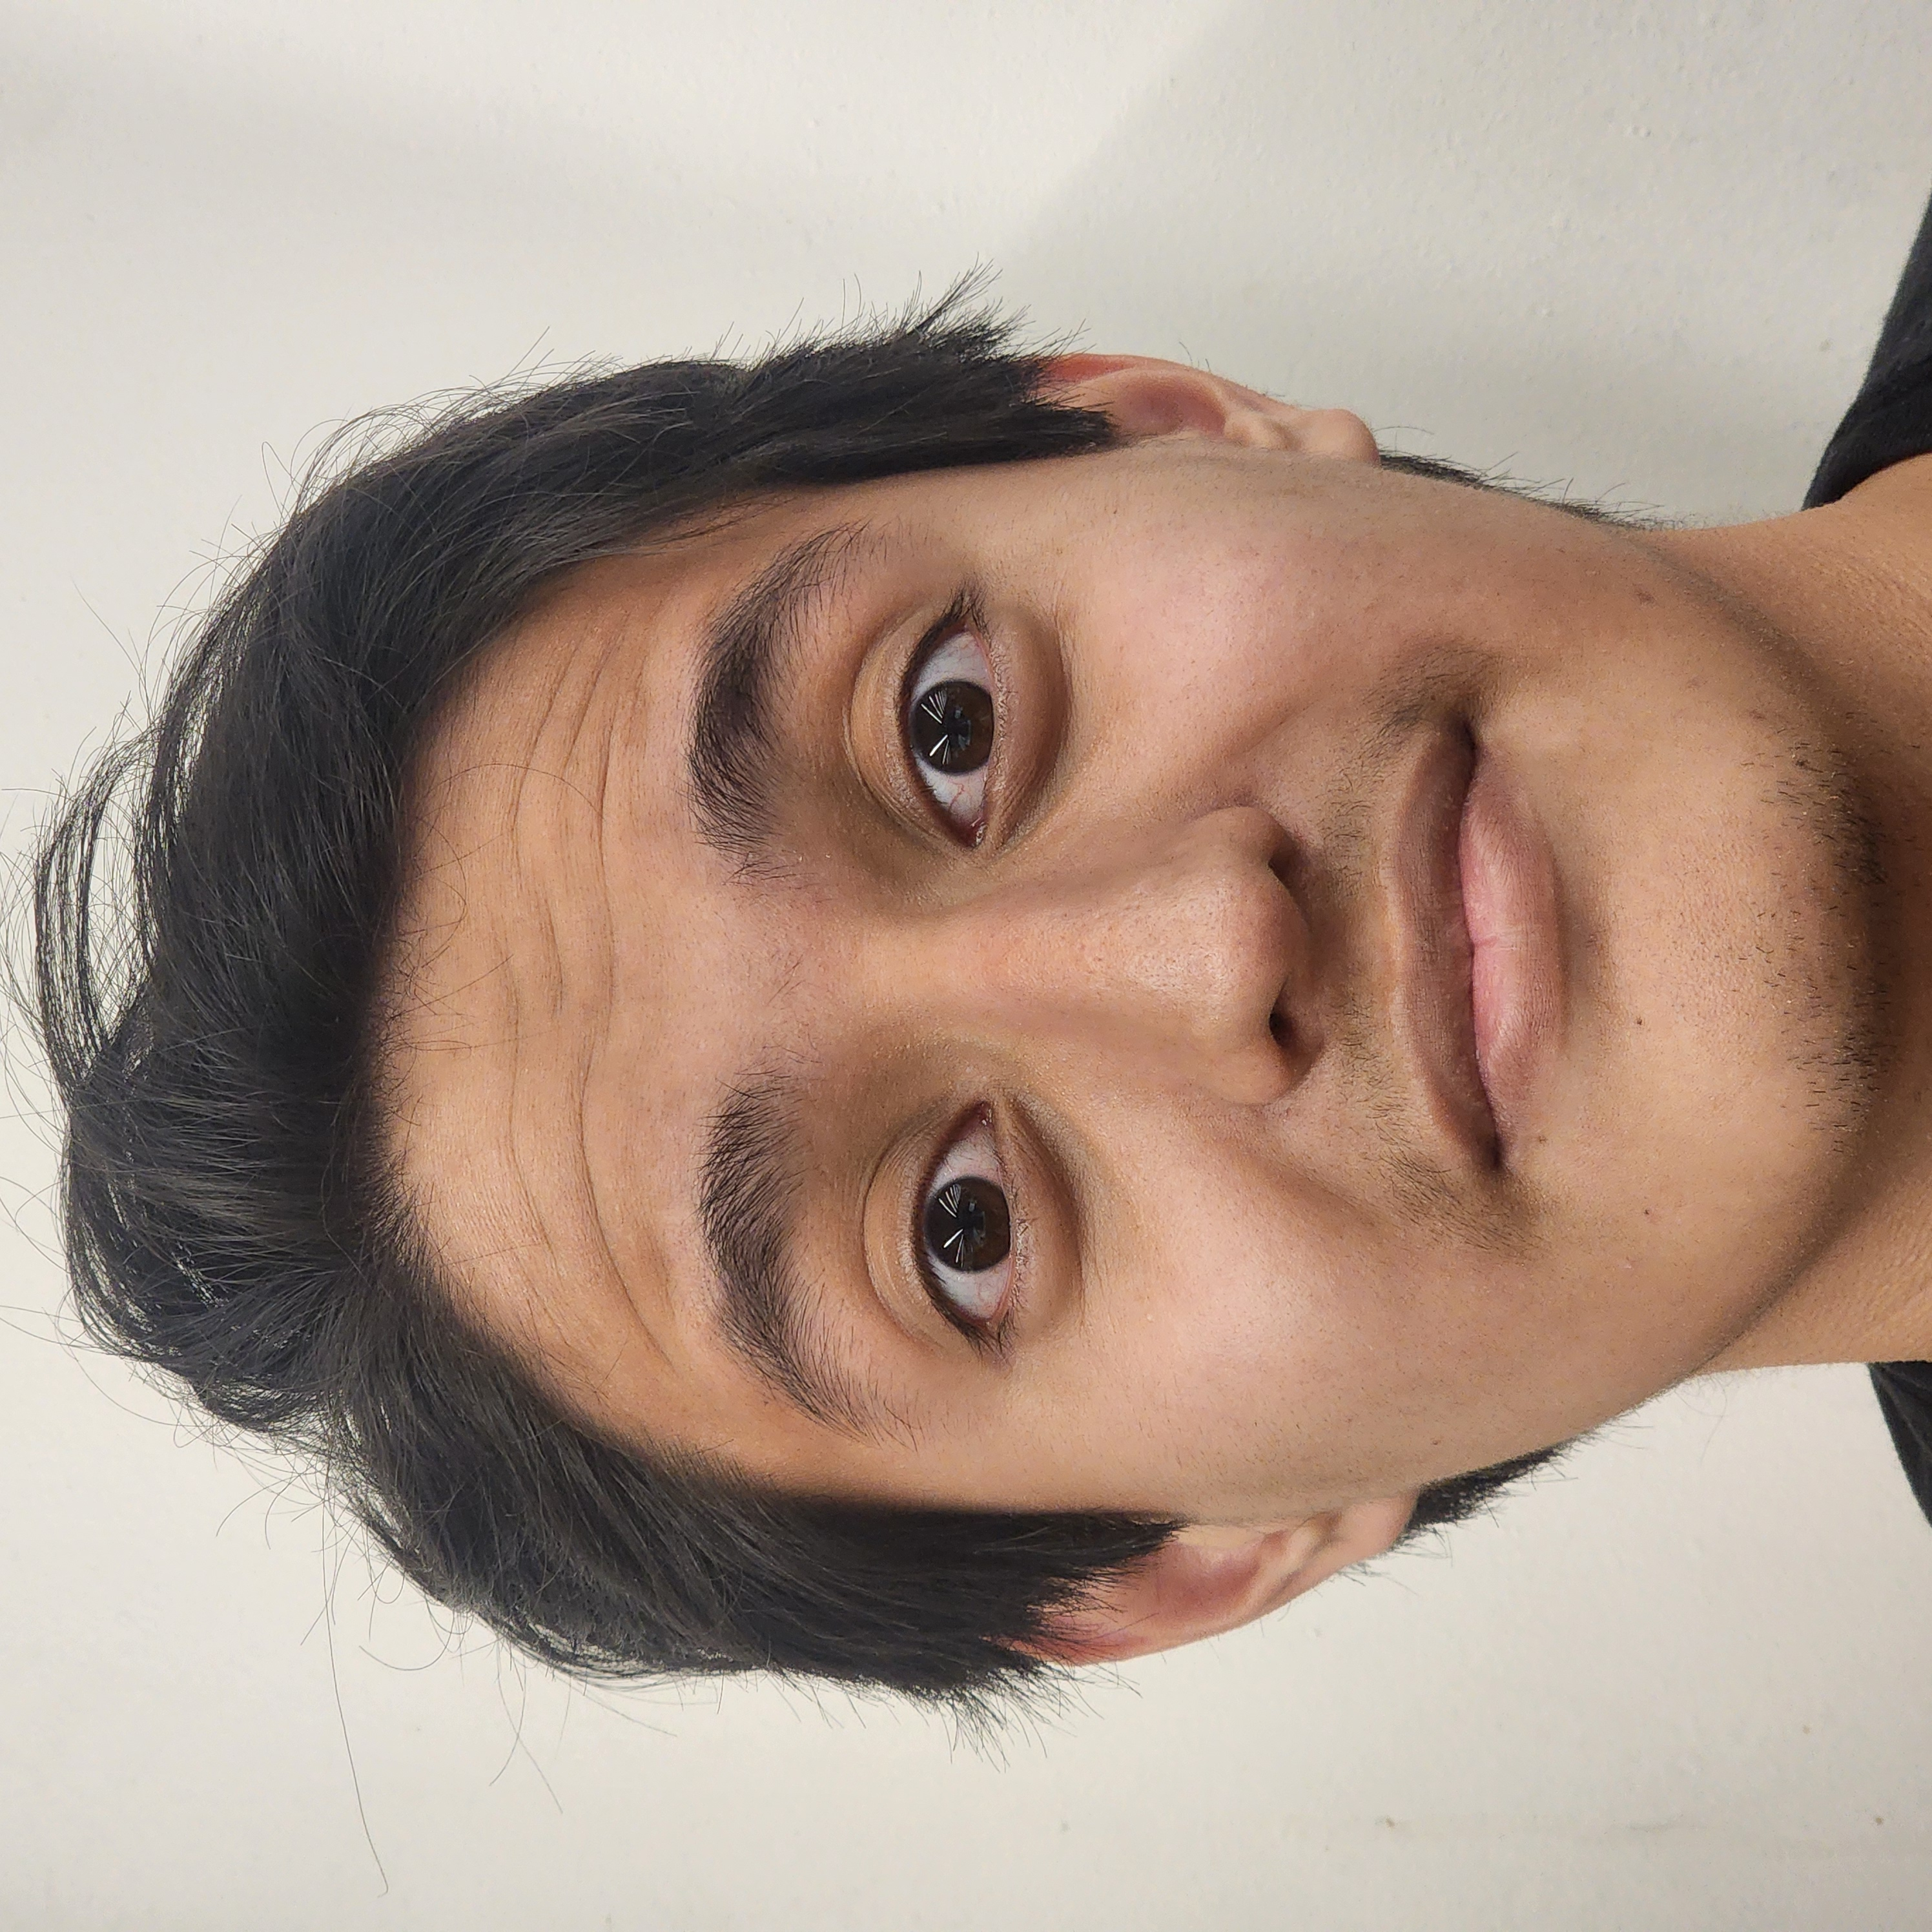
\includegraphics[width=\textwidth, angle=-90]{antes.jpg}
        \caption{Antes}
    \end{subfigure}
    \hfill
    \begin{subfigure}{0.3\textwidth}
        
\includegraphics[width=\textwidth]{despues.jpg}
        \caption{Después}
    \end{subfigure}
    \caption{Ejemplo de recorte facial 1.}
\end{figure}

% =========================
\section{Cumplimiento de la rúbrica}
% =========================

\subsection{Resumen de avance}
La Tabla~\ref{tab:rubrica} resume qué criterios están completos, parciales o pendientes con base en el código actual.

\begin{longtable}{p{1.2cm} p{6cm} p{3cm} p{4.2cm}}
\caption{Resumen de cumplimiento de la rúbrica.}
\label{tab:rubrica}\\
\toprule
\textbf{\#} & \textbf{Criterio} & \textbf{Estado} & \textbf{Comentario} \\
\midrule
\endfirsthead
\toprule
\textbf{\#} & \textbf{Criterio} & \textbf{Estado} & \textbf{Comentario} \\
\midrule
\endhead

1 & Diagnóstico de multicolinealidad con valores numéricos & Parcial & Se explica el problema, pero faltan VIF o correlaciones calculadas. \\
2 & Explicar por qué OLS falla & Completo & Incluido conceptualmente. \\
3 & Derivación analítica de Ridge & Completo & Se desarrolla paso a paso. \\
4 & Justificación geométrica & Parcial & Explicación textual; falta figura. \\
5 & Explicar el símplex regular & Completo & Incluido en teoría. \\
6 & Regla de clasificación y relación probabilística & Parcial & Regla incluida; falta profundizar Bayes. \\
7 & Pipeline completo y bias-variance & Completo & Incluido. \\
8 & Dataset sintético reproducible & Pendiente & No implementado en el código mostrado. \\
9 & Rasterización paramétrica & Pendiente & No implementado en el código mostrado. \\
10 & Split 80/20 + normalización correcta & Completo & Se implementó separación estratificada train/validation/test y normalización sin fuga de información. \\
11 & Ridge manual + barrido de alphas & Completo & Implementado. \\
12 & Ridge multivariado con símplex & Completo & Implementado. \\
13 & Ridge path & Completo & Implementado. \\
14 & MSE vs alpha en validación & Completo & El hiperparámetro $\alpha$ se seleccionó usando únicamente el conjunto de validación. \\
15 & Matriz de confusión y análisis & Parcial & Figura sí; falta análisis más detallado de identidades confundidas. \\
16 & Originales vs reconstruidas & Parcial & Hay visualización de test, pero no reconstrucción explícita. \\
17 & Accuracy vs nivel de ruido sigma & Pendiente & No implementado. \\
18 & Código limpio y modular & Parcial & Modular sí, faltan docstrings formales. \\
19 & Protocolo de captura documentado & Completo & Se describió el setup y se incluyó evidencia visual del entorno de captura. \\
20 & Consistencia de pose y 120 imágenes brutas & Parcial & Depende del dataset; falta documentar con mayor detalle el número bruto por identidad. \\
21 & Log de descartes & Completo & Se generó archivo CSV con nombre de archivo, motivo del descarte y fecha. \\
22 & Recorte y alineación con landmarks & Parcial & Hay recorte, pero no landmarks. \\
23 & Normalización de pixel + histogramas & Parcial & Se hace gris/resize, pero faltan histogramas comparativos. \\
24 & Data augmentation controlado & Pendiente & No implementado. \\
\bottomrule
\end{longtable}

% =========================
\section{Reflexión final}
% =========================
El desarrollo realizado permitió implementar el núcleo funcional del clasificador con Ridge Regression, incluyendo las partes más importantes del pipeline computacional: preprocesamiento, normalización, reducción de dimensionalidad, regularización, selección de hiperparámetro y clasificación multiclase basada en símplex regular. Además, se avanzó en la preparación de imágenes reales con una etapa de limpieza y recorte facial automatizado.

Sin embargo, al contrastar la implementación con la rúbrica, identificamos áreas pendientes. En el eje de teoría, faltan evidencias cuantitativas de multicolinealidad y una figura geométrica más clara. En programación, aún no se implementa la generación del dataset sintético, la rasterización paramétrica ni el experimento de sensibilidad al ruido. En el eje de captura y limpieza, se documentó el protocolo fotográfico, se incluyó evidencia visual del setup y se generó un archivo CSV con el registro de imágenes descartadas. Sin embargo, aún puede mejorarse el alineamiento facial mediante landmarks y la incorporación de histogramas comparativos antes y después del preprocesamiento.

Como plan de mejora, proponemos:
\begin{enumerate}
    \item implementar alineación facial basada en landmarks,
    \item incorporar histogramas comparativos antes y después del preprocesamiento,
    \item integrar el experimento de sensibilidad respecto a $\sigma$,
    \item implementar aumento de datos controlado,
    \item añadir dataset sintético paramétrico como comparación experimental.
\end{enumerate}

Consideramos que la entrega actual demuestra avance sustancial, comprensión del método y código ejecutable en las secciones declaradas como implementadas.

% =========================
\section{Conclusiones}
% =========================
Se implementó exitosamente un clasificador multiclase basado en Ridge Regression manual, con una estrategia geométrica de codificación por símplex regular. El modelo incluye normalización correcta, PCA, selección de hiperparámetro y evaluación visual y cuantitativa. Asimismo, se desarrolló una herramienta inicial para limpieza de imágenes reales.


% =========================
\section*{Apéndice A --- Repositorio del proyecto}
% =========================
Github del proyecto: \url{https://github.com/Cuper245/modulo3-munoz}
\end{document}